% !TEX root = ../thesis-main.tex

\chapter{Intent, Behavior and Satisfaction}
\label{chapter:research-intent}

\begin{figure}[ht]
  \centering
  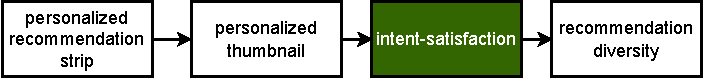
\includegraphics{images/pipeline_step3.pdf}
  \caption{The third step of the personalization pipeline}
  \label{fig:pip3}
\end{figure}

\footnote[]{This chapter was published at the ACM Transactions on Recommender Systems (TORS) under the title ``Intent-Satisfaction Modeling: From Music to Video Streaming'' \citep{intent}}
\acresetall

%\todo{Add intro paragraph that connects this chapter to its RQ from chapter 1: (How) Can we develop an explanation method based on a real-world use case and evaluate it in a human-centric way?  (Yes), we took a use case from Ahold and developed an explanation method around those users' needs. We evaluate the method with a user study that has objective + subjective components.}

In this chapter, we address the following research question:

\medskip
\noindent
\textbf{\ref{rq:intent}:} \acl{rq:intent}
\medskip

\noindent

\subimport{intent-based/intentBased/sections}{01-introduction}
\subimport{intent-based/intentBased/sections}{06-related-work}
\subimport{intent-based/intentBased/sections}{02-background}
\subimport{intent-based/intentBased/sections}{03-method}
\subimport{intent-based/intentBased/sections}{04-data-analysis}
\subimport{intent-based/intentBased/sections}{05-experimental-results}
\subimport{intent-based/intentBased/sections}{07-conclusions}


\begin{appendices}
\chapter{Appendix of Intent, Behavior and Satisfaction}
\subimport{intent-based/intentBased/appendix}{appendix}
\end{appendices}




\section*{Reproducibility}
To facilitate the reproducibility of the work in this chapter, our code is available at \url{https://github.com/rtlnl/streaming-intent-model}.